\section{Main result and its relation to the supplied work}
\label{sec:overview}

The main advance is an exact threshold for how many zero contributions
can simultaneously look alike after their sum is forced to be very small.
It is a structural theorem about the probability model attached to the
completed $L$-function. The zeros themselves are deterministic; all
randomness below comes from explicitly introduced gamma variables.

For a first reading, take the positive ordinates $\gamma_j$ of the zeros
of $\zeta$, including multiplicity, and independent exponential variables
$G_j$ of mean one. Put
\[
 X=\sum_j\frac{G_j}{\gamma_j^2},\qquad
 x=\sum_j\frac1{\gamma_j^2+u^2}.
\]
The second equation chooses $u=u(x)$ uniquely, with $u\to\infty$ as
$x\downarrow0$. Under RH the exact identity
\begin{equation}\label{eq:overview-transform}
 \mathbb E e^{-tX}
 =\frac{\xi(1/2)}{\xi(1/2+\sqrt t)},\qquad
 \xi(s)=\tfrac12s(s-1)\pi^{-s/2}\Gamma(s/2)\zeta(s),
\end{equation}
identifies this as the reciprocal-$\xi$ law studied in the article.
The same construction applies to a primitive real Dirichlet character
after removing any central zero factor. Nonreal characters are treated
by pairing the completed function with its conjugate.

The new sharp scale is
\begin{equation}\label{eq:overview-height}
 h_*(u)=\left(\frac{u^4}{\log u}\right)^{1/5}.
\end{equation}
Condition on $X\le x$ and observe the vector
$\bigl(u^2G_j/\gamma_j^2\bigr)_{\gamma_j\le h}$. Compare it with a
vector of independent exponential variables of mean one of the same
dimension. At $h=ch_*(u)$ the total-variation distance tends to
\begin{equation}\label{eq:overview-TV}
 \boxed{\quad 2\Phi\!\left(\frac{c^{5/2}}{\sqrt{50\pi}}\right)-1.\quad}
\end{equation}
Here $\Phi$ is the standard normal distribution function and the
total-variation distance is normalized to lie in $[0,1]$. The distance
tends to zero when $h/h_*(u)\to0$, and to one when $h/h_*(u)\to\infty$.
For example the limiting distances at $c=1,2,3,4$ are approximately
$0.06359,0.34826,0.78642,0.98933$.

This is stronger than convergence of any fixed collection of
coordinates. Every one of the individual rate corrections can tend to
zero while the joint vector becomes almost perfectly distinguishable
from the equal-rate product. The accumulated squared corrections,
rather than the largest correction, determine the transition. If
$n=N(u)$ is the number of positive ordinates below the saddle height,
the threshold contains order $n^{4/5}$ coordinates.

There is a second, larger scale. If each coordinate retains its actual
tilted rate $1+(\gamma_j/u)^2$, independence is valid in total variation
precisely for blocks with $h=o(u)$. At a positive fraction of $u$, the
small-sum constraint creates a nonzero limiting dependence, measured by
an explicit Gaussian overlap. These two thresholds separate the cost of
discarding small rate differences from the cost of discarding the
constraint on the total.

\begin{figure}[htbp]
 \centering
 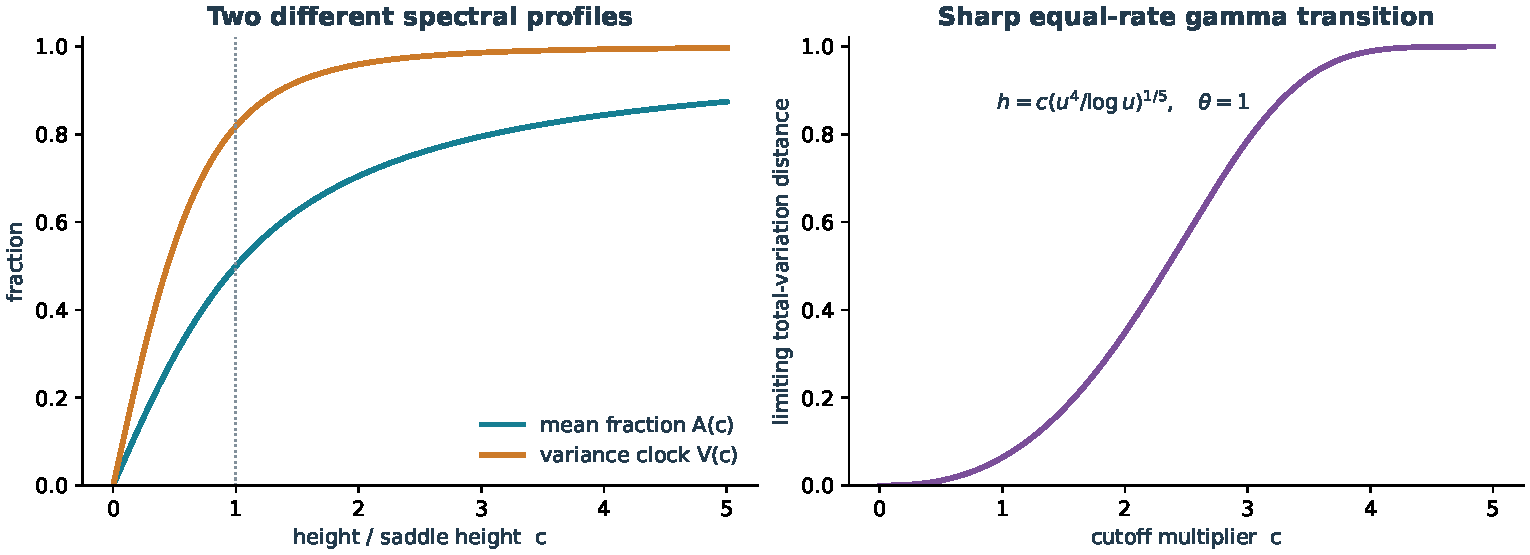
\includegraphics[width=\textwidth]{figures/universal_profiles.pdf}
 \caption{The mean allocation and fluctuation clock are different
 functions. The right panel shows the exact limiting distance in
 \eqref{eq:overview-TV}; these are analytic curves, not fitted data.}
 \label{fig:profiles}
\end{figure}

The proof also gives the conditional fraction contributed by ordinates
below $cu$:
\[
 \frac1X\sum_{\gamma_j\le cu}\frac{G_j}{\gamma_j^2}
 \longrightarrow A(c)=\frac2\pi\arctan c,
\]
uniformly in $c$ in probability. Thus half the contribution comes from
below the saddle height at first order. Its precise median height has a
systematic displacement of order $u/\log u$ and random fluctuations of
order $\sqrt{u/\log u}$. Section~\ref{sec:median} identifies both.

\subsection{What the source supplies}

The repository was pinned at commit
\texttt{2a9f8e3ee74a1824d57546f0b1b4f1cef5df93d6}.
Its vendored \texttt{Main.lean} exports Mathlib's ordinary
\texttt{RiemannHypothesis}, together with zero-free-half-plane and
critical-line theorems for Dirichlet $L$-functions~\cite{ProveItLean}.
The relevant GRH is the Dirichlet statement. A separate upstream
verification page reports kernel and external-checker verification of
the five theorem statements~\cite{Sutherland}.

The article's section \texttt{ana:sec:smalldev}, especially
\texttt{ana:thm:gammasum} and \texttt{ana:thm:smalldev}, supplies the
gamma series, its completed-function transform, and a detailed scalar
lower-tail asymptotic~\cite{ProveItArticle}. Its proof uses exponential
tilting and a local Gaussian limit for the total. The present work
extends that argument to independent spectral bands, to the exact
conditional density, and then to blocks whose dimension grows. The
arithmetic input is the completed-function identity and the classical
zero-counting formula. The new probability theorem is proved
independently under regular variation and does not use other unverified
claims from the merged article.

\subsection{Novelty and limits}

The reciprocal-$\xi$ law and the use of Hadamard products in probability
are established ideas~\cite{RoynetteYor,GaoHannigLeeTorcaso}. Conditioning
small Gaussian norms and conditional bridge limits for weighted sums
also have classical precedents~\cite{MayerWolfZeitouni,SobolevShklyaev}.
Sra's Appendix~C.17 contains a tilted Gaussian analysis for the
reciprocal-$\xi$ density~\cite{Sra}. We claim none of those mechanisms
as new.

The contribution developed here is the joint spectral conditional law,
the sharp growing-block total-variation transition and its explicit
four-fifths arithmetic specialization, the distinct macroscopic
independence transition, and the corrected median-height limit.
These results were not located in the inspected article or its seven
current incoming packets. The literature search found related general
conditioning results, but not these exact arithmetic statements. This
establishes a concrete extension of the supplied work; it does not
establish publication priority against all possible prior literature.

All new results have complete written proofs in this report. They have
not been formalized in Lean. The numerical artifacts illustrate finite
models and verify constants; they are not substitutes for the proofs.

